\documentclass[tikz=true]{standalone}
\usepackage{graphicx, standalone}
\usepackage[compat=1.1.0]{tikz-feynman}
\usepackage{tikz}
\usepackage{amsmath, amssymb}
\usepackage{euler}
\usepackage{fontspec}
\setmainfont{MinionPro}

\renewcommand{\k}{\ensuremath\text{k}}
\newcommand{\kp}{\ensuremath\text{k}'}
\newcommand{\q}{\ensuremath\text{q}}

\begin{document}

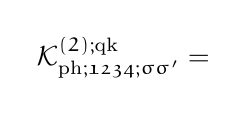
\begin{tikzpicture}[baseline=(current bounding box.center)]
	\node {$\mathcal{K}^{(2);\q\k}_{\text{ph};\mathfrak{1234};\sigma\sigma'}=$};
\end{tikzpicture}
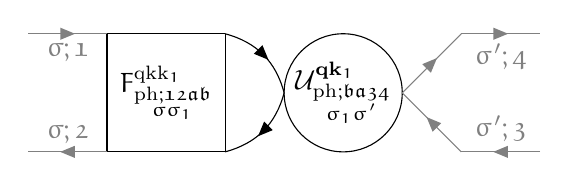
\begin{tikzpicture}[baseline=(current bounding box.center)]
	\begin{feynman}[small]
		\vertex (e1);
		\vertex[below=1.5cm of e1] (e2);
		\vertex[right=1.5cm of e1] (f1);
		\vertex[right=1.5cm of e2] (f2);
		
		\vertex (g) at ($(f1)+(0.75,-0.75)$);
		\vertex[right=1.5cm of g] (h);
		\vertex (i1) at ($(h)+(0.75,0.75)$);
		\vertex[below=1.5cm of i1] (i2);
		\vertex[right=of i1] (j1);
		\vertex[right=of i2] (j2);
		
		\vertex[left=of e1] (d1);
		\vertex[left=of e2] (d2); 
		
		\node at ($(e1)!0.5!(f2)$) {$F^{\q\k\k_1}_{\substack{\text{ph};\mathfrak{12ab}\\\sigma\sigma_1}}$};
		\node (u1) at ($(g)!0.5!(h)$) {$\mathcal{U}^{\textbf{q}\textbf{k}_1}_{\substack{\text{ph};\mathfrak{ba34}\\\sigma_1\sigma'}}$};
		
		\draw (u1) circle (0.75);		
		
		\diagram* {
			(e1) -- (f1) -- (f2) -- (e2) -- (e1),
			(f1) -- [fermion, bend left=30] (g) -- [fermion, bend left=30] (f2),
			(j2) -- [gray, fermion, edge label'=$\sigma';\mathfrak{3}$] (i2) -- [fermion, gray] (h) -- [fermion, gray] (i1) -- [gray, fermion,edge label'=$\sigma';\mathfrak{4}$] (j1),
			(d1) -- [gray, fermion, edge label'=$\sigma;\mathfrak{1}$] (e1),
			(e2) -- [gray, fermion, edge label'=$\sigma;\mathfrak{2}$] (d2),
		};
	\end{feynman}
\end{tikzpicture}
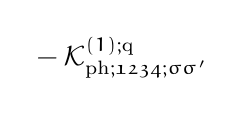
\begin{tikzpicture}[baseline=(current bounding box.center)]
	\node {$-\:\mathcal{K}^{(1);\q}_{\text{ph};\mathfrak{1234};\sigma\sigma'}$};
\end{tikzpicture}


\end{document}